\chapter{Fundamentação Teórica}
\label{cha:fundTeorica}

Esta seção apresenta uma fundamentação teórica básica sobre Computação Paralela sob
o ponto de vista arquitetural (Seção~\ref{sec:arquiteturas}) e de programação (Seção~\ref{sec:prog-paralela}).
Posteriormente, serão apresentados os conceitos fundamentais do padrão \stencil (Seção~\ref{sec:stencil}) e
sobre o \fw \pskel (Seção~\ref{sec:pskel}).

\section{Arquiteturas Paralelas}
\label{sec:arquiteturas}

De acordo com Tanenbaum~\etal~\cite{Tanenbaum2015}, as arquiteturas paralelas podem ser classificadas em
dois grandes grupos: multiprocessadores e multicomputadores. Nas seções a seguir são apresentados os
principais conceitos básicos destas duas classes de arquiteturas paralelas. Posteriormente, será discutido
em mais detalhes o processador \textit{manycore} \mppa, o qual será utilizado neste trabalho.

% \todo[inline]{Para o restante desta seção, tu podes pegar informações do livro do Tanenbaum de SO. O capítulo 8
% trata sobre multiprocessadores (seção 8.1) e multicomputadores (seção 8.2)}

\subsection{Multiprocessadores}

% \todo[inline]{
% - Organização: processadores interconectados a uma memória compartilhada via barramento (UMA). Podes usar a figura
% 8.2c do livro como base para fazer uma tua e mostrar as ideias.
% }

% \todo[inline]{
% - Podes falar rapidamente sobre NUMA e as diferenças para o UMA.
% }

% \todo[inline]{
% - Então, podes entrar no assunto dos multicores:

Multiprocessadores são sistemas constituídos de uma ou mais \cpus que
compartilham totalmente
a \ram do sistema. Desta forma, \textit{threads} de um mesmo processo se
comunicam através do mesmo espaço de endereçamento, por meio de escrita e
leitura na memória. Essa característica do sistema pode ocasionar problemas de
concorrência, onde um valor escrito por uma \textit{thread}, localizado em uma
palavra na memória, pode ser alterado por outra \textit{thread}, trazendo
inconsistência ao sistema.

Mais especificamente, multiprocessadores podem possuir propriedades adicionais,
como acesso uniforme à memória. Máquinas com essa propriedade são chamadas de
\uma. Por outro lado, existem multiprocessadores que não apresentam essa
característica, como é o caso de multiprocessadores \numa, que apresentam um acesso
não-uniforme à memória.

%\todo[inline]{\uma e \numa aparecem aqui pela primeira vez mas o nome não ficou por extenso.
%verificar o que está acontecendo...}

A Figura~\ref{fig:uma} apresenta a arquitetura de sistemas multiprocessados \uma
mais simplificados, onde existem várias \cpus que se
comunicam com uma memória compartilhada por meio de um barramento. Quando uma
\cpu deseja efetuar a comunicação, o barramento é verificado para
determinar a sua disponibilidade. Caso o barramento esteja ocupado, a
\cpu espera até que ele fique livre. Com o barramento livre, a \cpu
coloca o endereço da palavra no barramento, utiliza sinais de
controle e espera até que a memória coloque a palavra desejada no barramento. Esse
método é gerenciável para poucas \cpus, contudo com uma maior quantidade, o
número de comunicações aumenta significativamente, tornando
o gerenciamento de comunicações, por meio do barramento, insuportável. Desta
forma, o barramento se torna o gargalo do sistema.

\begin{figure}[t]
	\centering
    \caption{Esquema genérico de um multiprocessador \uma.}
    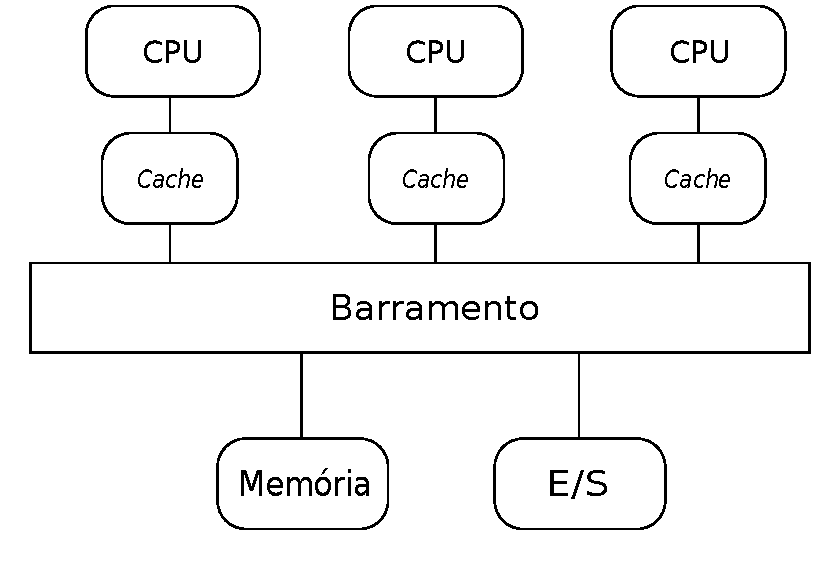
\includegraphics[width=0.5\textwidth]{figs/multiproc.pdf} \\
    Fonte: desenvolvido pelo autor.
    \label{fig:uma}
\end{figure}

A solução é utilizar \textit{caches} nas \cpus, possibilitando que requisições
de leitura sejam satisfeitas pela \textit{cache}, diminuindo a quantidade de
comunicações. Desta forma, é possível adicionar mais \cpus no barramento devido à baixa
quantidade de tráfego. \textit{Caches} possuem protocolos de coerência para
manter a consistência do sistema. Quando uma \cpu
efetua uma escrita sobre uma palavra, todas as \textit{caches} que possuem essa
palavra serão notificadas. Uma \textit{cache} com uma cópia modificada, isto é,
diferente do dado presente na memória, deve escrever essa cópia diretamente na
memória. Caso uma cópia exata do dado na memória esteja presente na
\textit{cache}, ela pode ser descartada, fazendo com que a \cpu acesse
diretamente a memória.

Além disso, é possível inserir mais níveis de \textit{cache} nas \cpus,
diminuindo o tráfego e retirando a necessidade de mais acessos à memória
principal. Contudo, devido ao limite arquitetural, uma quantidade muito grande
de \textit{caches} é inviável. Além disso, um tamanho muito grande para
\textit{caches} torna o seu acesso muito lento, prejudicando o desempenho do
sistema.

Sistemas multiprocessados \numa são diferentes de sistemas \uma, como mencionado
anteriormente, devido ao acesso à memória remota ser mais lento que à memória
local. A Figura~\ref{fig:numa} apresenta a arquitetura desse sistema, onde
existem nós interconectados por uma rede, e cada nó possui uma \cpu e um bloco
de memória. A \cpu de cada nó pode possuir uma \textit{cache}, denominada
\ccnuma, que possibilita uma redução no tempo de acesso a um dado localizado em
uma memória remota. Por outro lado, um sistema sem \textit{cache} é
denominado \ncnuma.

\begin{figure}[t]
	\centering
    \caption{Esquema genérico de um multiprocessador \numa.}
    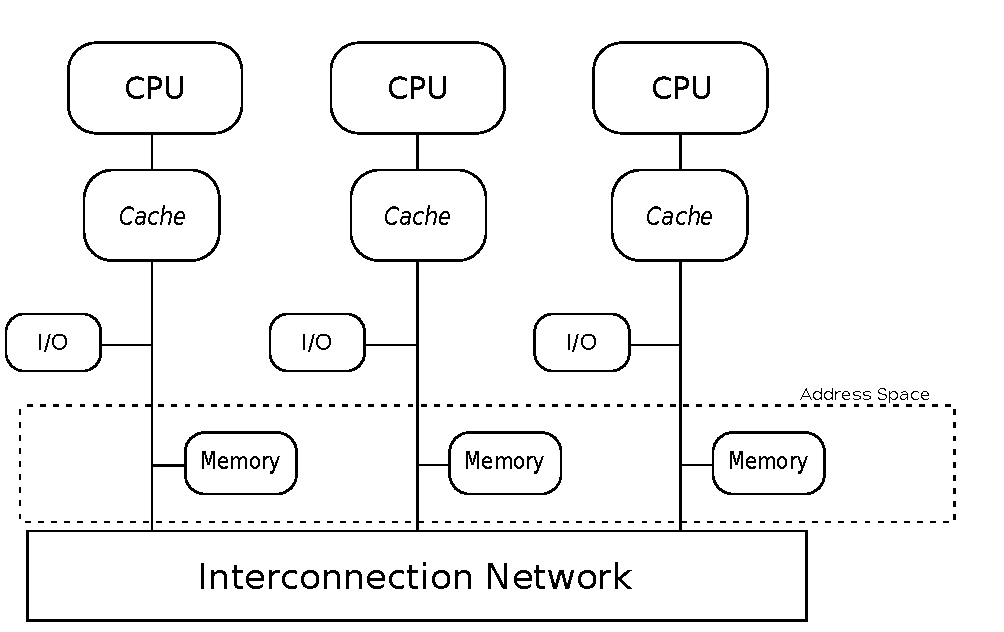
\includegraphics[width=0.6\textwidth]{figs/multiprocNUMA.pdf} \\
    Fonte: desenvolvido pelo autor.
    \label{fig:numa}
\end{figure}

Com o desenvolvimento de novas tecnologias, o tamanho
dos transistores diminuiu significativamente, se tornando possível inserir um
grande número de transistores em um único \textit{chip}.
Com o aumento da quantidade de transistores, um \textit{chip} pode ter, por
exemplo, várias \cpus (núcleos), caracterizando um
\textit{chip} \textit{multicore}.
Geralmente chamados de \cmps, os \textit{multicores} são semelhantes aos multiprocessadores
tradicionais, contudo, devido à proximidade de conexão entre \cpus, falhas em um
componente pode ocasionar problemas em outros componentes do sistema.
Esse problema pode ser ainda mais agravado em sistemas do tipo \mpsoc. Esses sistemas
possuem geralmente \cpus (muitas vezes \textit{multicore}) de propósito geral, além de processadores
dedicados a atividades bem específicas, tais como decodificadores de áudio e vídeo, processadores
criptográficos, entre outros. Além dos processadores, esses sistemas também incluem diferentes tipos
de interface de rede e de \es no mesmo \textit{chip}.

Quando a quantidade de núcleos é grande, isto é, dezenas ou milhares de
núcleos, o \textit{chip} pode ser classificado como \textit{manycore}.
Contudo, o limite para classificar um \textit{chip} em \textit{manycore} ou
\textit{multicore} é flexível~\cite{Tanenbaum2015}.
% Atualmente, aceleradores com uma grande quantidade núcleos estão
% surgindo, como o Xeon Phi da Intel com 60 núcleos.

Com vários núcleos em um único \textit{chip} problemas de coerência de
\textit{cache} começam a surgir. Mais especificamente, com o aumento no número
de núcleos, o custo sobre o protocolo de coerência vai crescer até que
aumentar o número de núcleos não auxiliará mais o desempenho, pois o sistema
estará gastando muito tempo mantendo as \textit{caches} consistentes.


Atualmente, sistemas computacionais comuns apresentam uma \gpu, onde temos
milhares de núcleos disponíveis. \gpus utilizam esses núcleos,
essencialmente, para a solução de cálculos, focando menos em questões de
\textit{cache} e lógica de controle. Desta forma, elas são utilizadas em
pequenas computações que podem ser paralelizadas. Contudo, a programação para
\gpus é difícil, pois os seus núcleos fazem a execução da mesma instrução
com diferentes partes do dado, isto é, são máquinas \simd. Esse modelo de
programação é interessante para abordar o paralelismo de dados, contudo, o
desenvolvedor pode se deparar com dificuldades durante o desenvolvimento.
Desta forma, linguagens de programação, como CUDA e \opencl,
abstraem o desenvolvimento de aplicações para esses processadores.

O \mppa é um processador \textit{manycore} diferente dos apresentados acima,
pois os seus núcleos são conectados atraves de uma \noc. Mais detalhes
sobre o \mppa serão apresentados posteriormente na Seção~\ref{sec:mppa}, tendo
em vista que ele possui também características relacionadas a multicomputadores.

% Até a última década, o desempenho sobre computadores escalava de acordo com o
% aumento da frequência dos processadores.
%
%
% Contudo, com o aumento da frequência,
% a potência e o consumo de energia também aumentam. De acordo com a
% Equação~\eqref{eq:power}, pode-se perceber que a potência aumenta,
% proporcionalmente, com o aumento da frequência.
%
%
% \begin{equation}\label{eq:power}
% 	P = CV^2f
% \end{equation}
%
% \todo[inline]{Esta parte está ruim. 1) Não foi explicada a equação (o que é P, C, V e f?).
% 2) Dizer que a potência aumenta proporcionalmente com o aumento da frequência não está totalmente correto,
% pois a tensão (V) também tem relação com a frequência (f). A tensão tem um impacto ainda maior, pois
% ela é quadrática na equação. Tens que dar uma olhada melhor nisso e corrigir o texto.}
%
% Portanto, o aumento do desempenho encontrou uma barreira no consumo de energia, onde tornou-se inviável
% um aumento indiscriminado da frequência. Desta forma, tornou-se necessário uma
% nova abordagem para aumentar o desempenho dos processadores. A solução encontrada
% pelos fabricantes de \textit{chips} foi de aumentar a quantidade de núcleos processamento no \textit{chip},
% porém reduzindo a frequência de operação dos mesmos, dando origem aos processadores \textit{multicore}.
%
% \todo[inline]{
% - Falar de \textit{manycores} (de modo geral), dando exemplos: Xeon Phi e GPU, que são dois tipos de \textit{manycores}
% bem diferentes.
% }
%
% \todo[inline]{
% - Finalizar dizendo que o \textit{manycore} utilizado neste trabalho se diferencia dos dois exemplos anteriores, pois
% seus núcleos são conectados através de uma NoC. Então, diz que será tratado desse assunto na Seção 2.1.3
% }
%
\subsection{Multicomputadores}

% \todo[inline]{
% - Organização: sistemas multiprocessados, cada um com sua memória de dedicada, conectados através de uma rede. Podes usar
% a figura 8-18 como base para explicar as ideias.
% }
%
% \todo[inline]{
% - Podes falar rapidamente dos diferentes tipos de interconexão: figura 8-16 do livro
% }
%
% \todo[inline]{
% - Falar dos tipos de multicomputadores: NOW, COW, etc...
% }
%
% \todo[inline]{
% - Finalizar indicando que nos multicomputadores a comunicação entre os processadores é feita de maneira explícita através de trocas de mensagens.
% }
%
Multiprocessadores de grande porte são difíceis de construir devido ao alto
custo. Desta forma, devido à simplicidade de construção, multicomputadores
começaram a surgir. A ideia principal de um multicomputador é agregar em um mesmo sistema diversos
computadores, os quais muitas vezes possuem multiprocessadores~\cite{Tanenbaum2015}.
Nesse sentido, um computador com sua placa de interface de rede é considerado como um nó do
sistema multicomputado, onde um gerenciamento de forma inteligente da rede auxilia o desempenho
do sistema.

\begin{figure}[t]
	\centering
    \caption{Esquema simples de um sistema multicomputado.}
        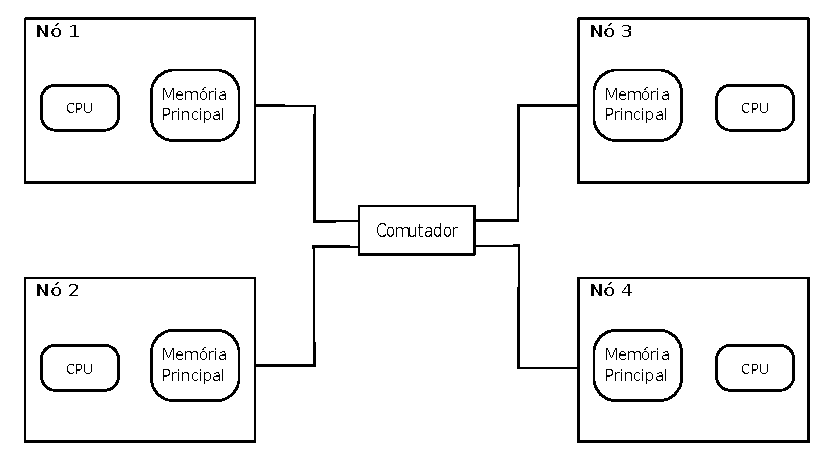
\includegraphics[width=0.7\textwidth]{figs/multicomp.pdf} \\
        Fonte: desenvolvido pelo autor.
        \label{fig:multicomputado}
\end{figure}



A Figura~\ref{fig:multicomputado} mostra como um sistema multicomputado simples é
organizado. Existem nós que possuem uma \cpu, memória principal dedicada e uma
conexão diretamente com outros nós ou a um comutador. A topologia apresentada na
imagem é uma das topologias possíveis em um sistema multicomputado. Outra
alternativa é utilizar uma topologia em anel (Figura~\ref{fig:topologia}b), retirando a necessidade de um
comutador, pois um nó é conectado diretamente aos outros nós. Cada nó é
conectado ao nó à sua esquerda e à sua direita.

Uma outra topologia de interconexão muito utilizada em multicomputadores é a malha (\textit{mesh}),
a qual é ilustrada pela Figura~\ref{fig:topologia}c. Nesse tipo de topologia, os nós são interconectados
em comutadores distintos pelo sistema e cada comutador é conectado a outros
comutadores, formando uma espécie de malha no sistema. Uma variante dessa
topologia é o toro duplo (\textit{torus}) apresentado na Figura~\ref{fig:topologia}d, onde os
comutadores de cantos opostos estão conectados diretamente. Desta forma,
comunicações entre nós de cantos opostos não terão a necessidade de inúmeros
saltos pelos comutadores para efetuar a transmissão de informações.

A Figura~\ref{fig:topologia}e ilustra uma topologia tridimensional, e a
Figura~\ref{fig:topologia}f ilustra um cubo tetradimensional. Topologias
$n$ dimensionais são utilizadas para diminuir o atraso de comunicação entre nós,
pois o diâmetro da rede cresce linearmente de acordo com a dimensionalidade.
Mais precisamente, o diâmetro da rede é o maior caminho entre dois nós e cresce
de acordo com a raiz quadrada do número de nós. Desta
forma, topologias $n$ dimensionais permitem que o diâmetro da rede seja menor,
mesmo com um número maior de nós.
Devido a essa propriedade, topologias $n$ dimensionais são utilizadas em
vários sistemas.

\begin{figure}[t]
	\centering
        \caption{Topologias de interconexão.}
	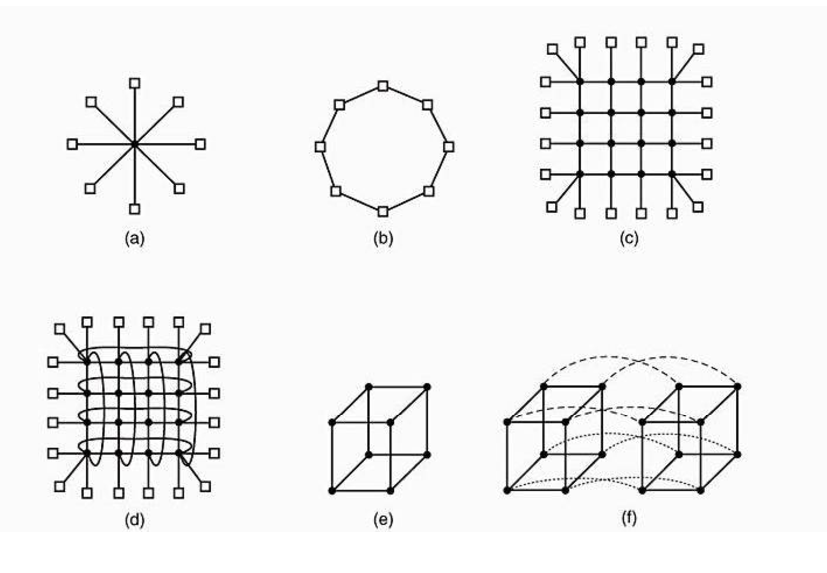
\includegraphics[width=\textwidth]{figs/topologia.pdf} \\
    Fonte:~\cite{Tanenbaum2015}
    \label{fig:topologia}
\end{figure}


%Cow Now
Geralmente, multicomputadores podem ser construídos com computadores pessoais
comuns interconectados por uma interface de rede para trabalharem em
conjunto. Organizações de multicomputadores deste tipo são denominadas de \now. Devido à sua
simplicidade, esse sistema não é focado em ganho de desempenho. Por outro lado, \cow
são constituídos de computadores interconectados sem teclado, monitor e \textit{mouse} contendo cada
um diversos processadores de alto desempenho. Esses sistemas são focados em desempenho, pois
possuem redes de interconexão de alto desempenho (alta largura de banda e baixa latência).

A comunicação em um multicomputador é feita por meio de troca de mensagens.
Processos localizados em diferentes \cpus se comunicam por meio de mecanismos básicos
disponibilizados pelo \so. Esses mecanismos básicos do \so são utilizados como base para implementação
de bibliotecas de comunicação que implementam, pelo menos, duas primitivas básicas: \textit{send} e \textit{receive}.
A primitiva \textit{send} envia uma mensagem para um processo, o que é determinado pelos
parâmetros de entrada da mesma. A primitiva \textit{receive} é responsável pelo recebimento
de mensagens, utilizando como parâmetro o endereço que será lido para coletar a
mensagem recebida. Portanto, em sistemas multicomputados a troca de mensagens
entre processos é realizada de maneira explícita pelo desenvolvedor.


\subsection{O Processador \textit{Manycore} MPPA-256}
\label{sec:mppa}

O \mppa é um processador \textit{manycore} desenvolvido pela empresa francesa
Kalray, o qual possui 256 núcleos de processamento de 400 MHz. Ele mistura características
de um multiprocessador e de um multicomputador, porém em um único \textit{chip}.
Mais especificamente, o \mppa utiliza um modelo multicomputado com uma
comunicação via \noc em seus \textit{clusters}, e um modelo multiprocessado
dentro de cada \textit{cluster}.

\begin{figure}[t]
	\centering
	\caption{Visão geral do \mppa.}
	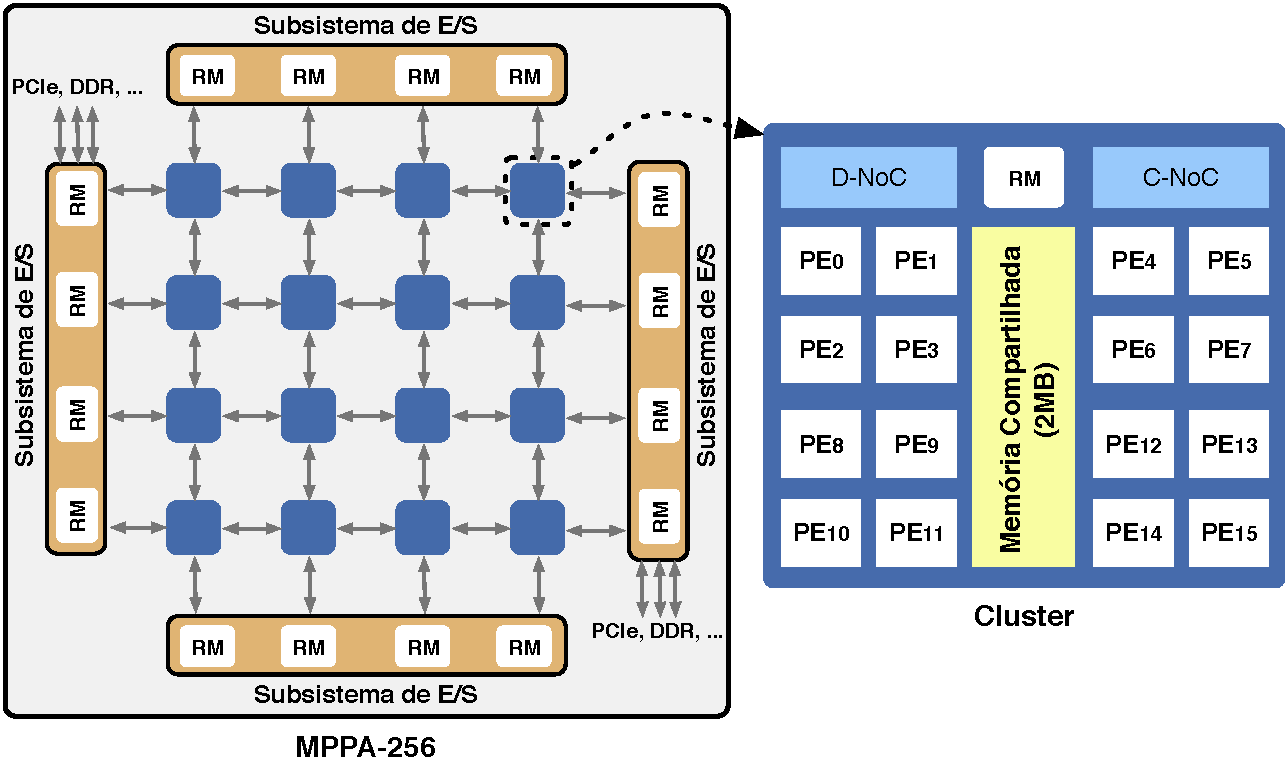
\includegraphics[width=0.9\textwidth]{figs/mppa-overall.pdf} \\
    Fonte:~\cite{Castro-IA3:2013}
	\label{fig:mppa}
\end{figure}

Os núcleos de processamento do \mppa são denominados \pes.
Além dos \pes, o processador possui 32 núcleos dedicados à gerência de recursos
denominados  \rmans. \pes e \rmans são distribuídos
fisicamente no \textit{chip} em 16 \textit{clusters} e 4 subsistemas de \es,
onde cada \textit{cluster} contém 16 \pes e 1 \rman. Além dos \textit{clusters}, o
\mppa possui 4 subsistemas de \es contendo, cada um, 4 \rmans. Toda a comunicação
entre \textit{clusters} e/ou subsistemas de \es é feita através de uma \noc
\textit{torus} 2D. A arquitetura do \mppa pode ser vista na
Figura~\ref{fig:mppa}\footnote{A figura apresenta uma ilustração simplificada,
    omitindo a topologia da \noc.}.

A finalidade principal dos \pes é executar \textit{threads} de usuário de forma
ininterrupta e não preemptível para realização de computação. \pes de um mesmo
\textit{cluster} compartilham uma memória de 2~\mb, a qual é utilizada para
armazenar os dados a serem processados pelos \pes. Cada \pe possui também uma
memória \textit{cache} associativa 2-\textit{way} de 32~\kb para dados e uma para
instruções. Porém, o processador não dispõe de coerência de \textit{caches}, o
que dificulta o desenvolvimento de aplicações para esse processador. Por outro
lado, a finalidade dos \rmans é gerenciar \es, controlar comunicações entre
\textit{clusters} e/ou subsistemas de \es e realizar comunicação com uma memória
\ram. Na arquitetura utilizada neste trabalho, um dos subsistemas de \es está conectado a uma
memória externa \lpddr de 2~\gb.

A comunicação dos \textit{clusters} com o subsistema de \es e a comunicação
entre \textit{clusters} é realizada de maneira explícita, utilizando uma \api
própria do \mppa de baixo nível similar à \posix \ipc. Detalhes referentes à
comunicação e programação nesse processador serão abordadas posteriormente
na Seção~\ref{sec:prog-mppa}.

% - Terminar essa seção falando que a comunicação entre clusters e entre cluster/IO tem
% que ser feita de maneira explícita utilizando uma API de baixo nível. Então, diz que os detalhes
% referentes a programação nesse processador serão tratados na Seção 2.2.3
%----------------------------------------------------------------------------------------
%Existem diversos tipos de arquiteturas que proporcionam ao desenvolvedor uma
%abordagem paralela. Multiprocessadores são arquiteturas que fornecem vários
%núcleos de processamento em uma máquina e a comunicação entre os núcleos é feita
%através da memória compartilhada, contudo este modelo traz dificuldades em
%relação à organização e particionamento de dados entre núcleos. Devido ao espaço
%limitado em \textit{chip}, o aumento do número de núcleos nessa arquitetura pode
%se tornar inviável, portanto, arquiteturas multicomputadas são utilizadas, onde
%temos várias máquinas, sendo, geralmente, multiprocessadas, interligadas para
%fornecer um maior poder de processamento. A comunicação entre cada
%\textit{cluster}, isto é, cada nó na rede de computadores utiliza distribuição
%de dados e sincronizações, como não temos compartilhamento de memória entre os
%nós de processamento, o desenvolvimento de código para essa arquitetura é mais
%complicada, pois existem vários fatores à serem avaliados pelo desenvolvedor. Na
%próxima seção serão abordadas as dificuldades e implementação de cada modelo.

%Arquiteturas paralelas: multicomputadores, multiprocessadores, compartilhamento de memória e distribuição de dados.
%Programação paralela: uso de apis, dificuldades. POSIX, MPI...


\section{Programação Paralela}
\label{sec:prog-paralela}

Aplicações são, geralmente, implementadas de forma
sequencial, isto é, um conjunto serializado de instruções que será executado
sobre uma \cpu. Por outro lado, a computação paralela ou distribuída efetua o
processamento de instruções sobre múltiplos elementos de processamento. A ideia
principal é dividir a computação em partes menores que podem ser executadas
simultaneamente entre os elementos de processamento distintos, com intuito de se
realizar um processamento em menos tempo.

Diferentes \apis de programação paralela foram criadas com intuito de simplificar
o desenvolvimento de aplicações em arquiteturas multiprocessadas e multicomputadas.
A seguir serão apresentadas as \apis mais utilizadas no âmbito de \hpc em cada tipo de
arquitetura. Por fim, será apresentada a \api utilizada para o desenvolvimento de aplicações
no processador \mppa.


\subsection{OpenMP}

% \todo[inline]{
% - Dizer que é feita para ser utilizada em arquiteturas multiprocessadas, ou seja, com memória
% compartilhada.
% }
%
% \todo[inline]{
% - Apresentar as principais ideias do OpenMP: dizer que é baseada em pragmas, modelo fork-join,
% regiões paralelas, paralelização de laços, ... (A \api é baseada no modelo de programação
% paralela de memória compartilhada, apresentando uma boa portabilidade e pouco
% esforço de programação. O modelo de programação utiliza diretivas de compilação
% e variáveis, tornando possível poucas modificações de código para utilizar
% outras \textit{threads} na aplicação....)
% }


Para evitar uma programação de baixo nível sobre um sistema multiprocessado, são
utilizadas \apis para o desenvolvimento de aplicações, como o OpenMP. O OpenMP
é um modelo de programação baseado em memória compartilhada e provê uma maior
facilidade no desenvolvimento de aplicações para o ambiente multiprocessado,
permitindo a paralelização de aplicações com variáveis de ambiente e
diretivas de compilação.

O OpenMP utiliza o modelo \textit{fork-join}, onde a execução inicia com uma
única \textit{thread}, denominada \textit{master thread}. Como ilustrado na
Figura~\ref{fig:forkjoin}, quando a \textit{master thread} encontra
uma região paralela, são criadas outras \textit{threads} de acordo com a variável
de ambiente especificada no sistema. No final da região paralela, é realizado um
\textit{join} por meio de uma barreira implícita, onde as \textit{threads} serão
sincronizadas, e a execução irá continuar apenas com a \textit{master thread}.

\begin{figure}[t]
	\centering
	\caption{Esquemático do modelo \textit{fork-join}.}
	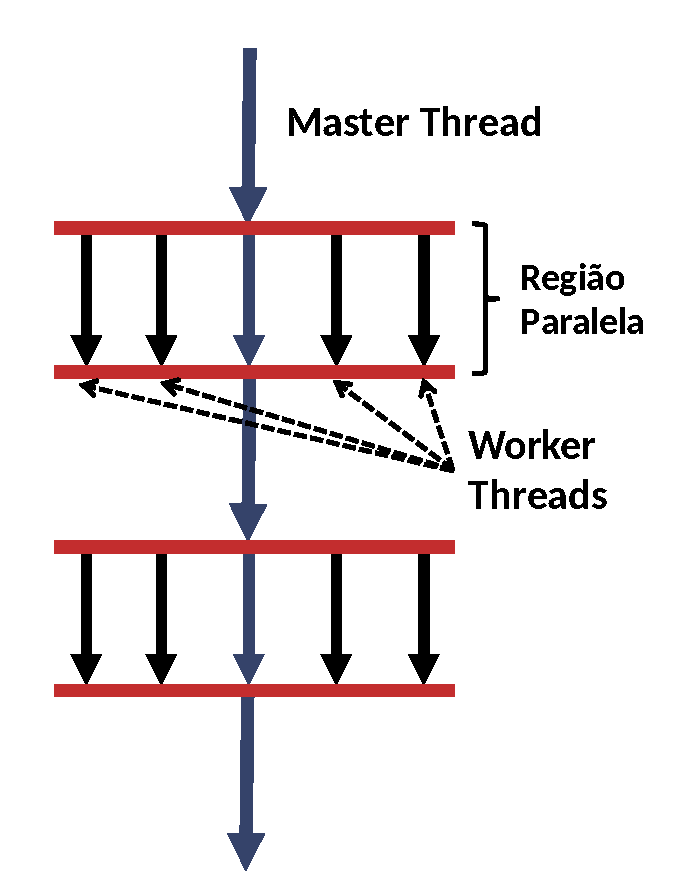
\includegraphics[width=0.4\textwidth]{figs/forkjoin.pdf} \\
    Fonte: desenvolvido pelo autor.
	\label{fig:forkjoin}
\end{figure}

Por meio de diretivas de compilação é possível definir o comportamento do
OpenMP, inclusive, determinar regiões paralelas e outras funções da \api.
O Código~\ref{cod:exemplo-openmp} apresenta um exemplo de uma função
que implementa o produto escalar entre dois vetores (\texttt{a} e \texttt{b}) paralelizada
com uso do OpenMP. A região paralela é criada pela diretiva de compilação
\texttt{\#pragma omp parallel} (linha 5). Variáveis dentro de uma região paralela
podem ser classificadas como \texttt{shared} (compartilhadas) ou \texttt{private} (privadas),
possibilitando assim o gerenciamento da execução pela \api. Uma variável marcada como \texttt{shared}
é compartilhada entre as \textit{threads} de uma região paralela. Por outro lado, variáveis marcadas
como \texttt{private} são privadas para cada \textit{thread}, isto é, cada \textit{thread} possuirá uma
cópia privada da variável. Desta forma, as modificações sobre elas serão feitas localmente em cada
\textit{thread}.

As diretivas do OpenMP, além de determinar regiões paralelas, possibilitam
paralelizar laços de maneira automática, onde as iterações
do laço são distribuídas, de forma automática e flexível, sobre as
\textit{threads} da região paralela. A paralelização das iterações do laço é mostrada na linha 6 do
Código~\ref{cod:exemplo-openmp} com uso da cláusula \texttt{for}. Além disso, operações de redução podem ser
utilizadas ao fim de uma região paralela, aplicando sobre uma variável a
operação especificada. Ao final da região paralela, o resultado é atribuído a uma variável compartilhada. A redução
é necessária no caso do produto escalar mostrado no Código~\ref{cod:exemplo-openmp}, sendo necessário
utilizar a cláusula \texttt{reduction} sobre a variável \texttt{prod}. A operação de redução utilizada no caso do produto
escalar é a soma (\texttt{+}).

\begin{figure}[t]
	\begin{lstlisting}[
		caption=Produto escalar paralelo com OpenMP.,
		label=cod:exemplo-openmp,
	]
	int produto_escalar(int *a, int *b, int tamanho)
	{
		int prod = 0;

		#pragma omp parallel for private(i) shared(a, b) \
                                        reduction(+:prod)
		for (int i = 0; i < tamanho; i++)
			prod += a[i] * b[i];

		return(prod);
	}
	\end{lstlisting}
\end{figure}

Devido à abstração que o modelo oferece, poucas modificações de código são
necessárias para paralelizar uma aplicação. \posix \textit{threads} é outro
modelo que pode ser utilizado, contudo com uma menor abstração que o modelo
OpenMP.

%Computação paralela em uma arquitetura multiprocessada contém diversas
%dificuldades para o desenvolvimento de código, como: \textbf{(i) dependência de
%    dados:} quando um processo ou \textit{thread} está executando uma parte do
%código, outra \textit{thread} deve ter os dados atualizados corretamente. Esta
%dependência pode gerar problemas, como \textit{deadlocks} e \textit{livelocks}.
%\textit{Deadlocks} são conflitos que ocorrem entre \textit{threads}, quando uma
%\textit{thread} $A$ precisa de um recurso alocado por uma \textit{thread} $B$
%que, por sua vez, precisa de um recurso alocado pela \textit{thread} $A$, ocorre
%um ciclo na execução, caracterizando um \textit{deadlock}. Por outro lado,
%\textit{Livelocks} são similares aos \textit{deadlocks}, contudo o estado das
%\textit{threads} estão em constante mudança, fazendo com que nenhum deles
%continue sua execução normalmente, pois a cada mudança um \textit{deadlock}
%ocorre. Além disso, dependências geram problemas de sincronização entre
%\textit{threads}, deixando para o desenvolvedor da aplicação a tarefa de
%gerenciar corretamente a execução. \textbf{(ii) Condição de Corrida:} uma
%\textit{thread} escreve sobre uma váriavel ou, mais especificamente, um espaço
%de memória, enquanto outra \textit{thread} fará alguma operação sobre esse mesmo
%espaço. Isso pode gerar inconsistências de dados, entre outros problemas.

\subsection{MPI}

% \todo[inline]{
% - Motivação para usar MPI:
%
% A programação paralela em multicomputadores é feita através da utilização de múltiplos processos que se comunicam
% através de trocas de mensagens. Devido à característica de baixo nível intrínseca do modelo de troca de
% mensagens, utilizar \textit{sockets} manualmente para a comunicação entre nós de
% uma rede de \textit{clusters} é inadequada para o desenvolvedor. Portanto, mostra-se necessário utilizar
% APIs de mais alto nível, possibilitando uma maior abstração ao desenvolvedor.
% }
%
% \todo[inline]{
% - Dizer que MPI é a API mais amplamente utilizada para programação paralela em multicomputadores, ou seja, para arquiteturas multicomputadas, ou seja, com memória distribuída.
% }
%
% \todo[inline]{
% - Apresentar as principais ideias do MPI: processos MPI, rank, Send/Recv, comunicações coletivas, ...
% }

A programação paralela em multicomputadores é feita através da utilização de múltiplos processos que se comunicam
através de trocas de mensagens. Devido à característica de baixo nível intrínseca do modelo de troca de
mensagens, utilizar \textit{sockets} manualmente para a comunicação entre nós de
uma rede de \textit{clusters} é inadequada para o desenvolvedor. Portanto, mostra-se necessário utilizar
APIs de mais alto nível, possibilitando uma maior abstração ao desenvolvedor.

O \mpi é uma \api utilizada amplamente em multicomputadores fornecendo uma maior
abstração em relação à programação sobre \textit{sockets}. A \api é baseada no
modelo \spmd, onde todos os processos executam o mesmo programa, porém cada processo é responsável
por realizar computações em dados distintos.

A \api fornece diversas funções aos desenvolvedores. A função \texttt{MPI\_Init()} permite inicializar o ambiente \mpi.
Após a inicialização, cada processo \mpi possuirá um identificador único (de $0$ até $np-1$, onde $np$ é o número total
de processos \mpi em execução). Esse identificador único, denominado \textit{rank}, poderá ser utilizado em conjunto com
instruções de seleção (\texttt{if-else}) para determinar que processos \mpi
distintos possam executar códigos distintos. Além disso,
ele será utilizado nas primitivas de comunicação do \mpi para especificar os remetentes e destinatários das mensagens.
Para finalizar o ambiente \mpi é feita uma chamada para a função \texttt{MPI\_Finalize()}. O envio de mensagens
é realizado pela função \texttt{MPI\_Send()}, que construirá a mensagem, e irá
adicionar o \textit{rank} do destinatário, o \textit{rank} do remetente, entre
outras informações. A função \texttt{MPI\_Recv()} será responsável por receber a
mensagem enviada pelo processo, e irá armazená-la no espaço de memória
do processo destinatário.

O Código~\ref{cod:exemplo-mpi} mostra um exemplo de um programa em \mpi. Nesse
exemplo, o processo com \textit{rank} igual a zero
envia uma mensagem a todos os demais processos. Ao receber a mensagem, cada um dos demais processos imprime na tela a mensagem
recebida. As funções \texttt{MPI\_Comm\_rank()} e \texttt{MPI\_Comm\_size()} são utilizadas para armazenar nas variáveis \texttt{rank} e \texttt{size}
o \textit{rank} do processo e o número total de processos, respectivamente. Nas
linhas 12-13, o processo com \textit{rank} igual a zero envia para os
demais processos a mensagem \texttt{``Ola mundo!''}. As linhas 16-19 são executadas somente pelos demais processos, onde cada processo
realiza o recebimento da mensagem e a imprime na tela juntamente com seu \textit{rank}.

\begin{figure}[t]
	\begin{lstlisting}[
		caption=Exemplo de um programa MPI.,
		label=cod:exemplo-mpi,
	]
	int main(int argc, char **argv)
	{
		int rank, size;

		MPI_Init(argc, argv);

		MPI_Comm_rank(MPI_COMM_WORLD, &rank);
		MPI_Comm_size(MPI_COMM_WORLD, &size);

		if (rank == 0) {
			char mensagem[11] = "Ola mundo!";
			for (int i = 1; i < size; i++)
				MPI_Send(&mensagem, 11, MPI_CHAR, i, 0, MPI_COMM_WORLD);
		}
		else {
			char mensagem[11];
			MPI_Recv(&mensagem, 11, MPI_CHAR, 0, MPI_ANY_TAG,
                             MPI_COMM_WORLD, MPI_STATUS_IGNORE);
			printf("Processo %d recebeu: %s\n", rank, mensagem);
		}

		MPI_Finalize();
		return(0);
	}
	\end{lstlisting}
\end{figure}

Além de comunicações do tipo ponto-a-ponto, existem comunicações coletivas e de sincronização entre
todos os processos. A função \texttt{MPI\_Barrier()} é uma barreira de sincronização, responsável por bloquear a
execução de um processo até que todos os outros processos cheguem na barreira.
Por outro lado, a função \texttt{MPI\_Bcast()} é responsável por enviar a mesma
mensagem de um processo para todos os outros processos do sistema de forma otimizada.

%
% \renewcommand{\lstlistingname}{Código}
% \definecolor{lightgray}{rgb}{0.97,0.97,0.97}
% \definecolor{lightred}{rgb}{1,0.7,0.7}
%
% \lstdefinelanguage{cc}{
%     language     = C++,
%     morekeywords = {Array2D, __parallel__, Mask2D, Stencil2D, pragma, omp, parallel, printf},
% }
%
% \lstset{
% numbers=none,
% stepnumber=1,
% numbersep=-8pt,
% numberstyle=\small\color{black},
% basicstyle=\scriptsize\ttfamily,
% keywordstyle=\color{blue},
% commentstyle=\color{black},
% stringstyle=\color{black},
% numberstyle=\footnotesize\ttfamily\color{black},
% escapeinside={(@}{@)},
% frame=none, %single
% tabsize=2,
% float,
% language=cc, %morecomment=[l][{\color[rgb]{0.1, 0.2, 0.8}}]{},
% %aboveskip=0.1in, % space before the caption
% %belowskip=0.1in, % space after listing
% captionpos=b,
% showstringspaces=false,
% %belowcaptionskip=1\baselineskip,
% %breaklines=true,
% %moredelim=[l][\color{blue}]{\#pragma},
% backgroundcolor=\color{white},
% %xleftmargin=.2\textwidth, xrightmargin=.2\textwidth
% }
%
% \begin{figure}[thp] % the figure provides the caption
% \centering          % which should be centered
% \begin{tabular}{c}
%
% \begin{lstlisting}[]
%     (@\textcolor{blue}{\#}@)pragma omp parallel
%     printf("Hello World!");
% \end{lstlisting}
% \end{tabular}
% \caption*{Exemplo de código OpenMP.}
% \end{figure}
%
% \todo{Apresentar código \MPI}


%Ao aperfeiçoar esses modelos, começaram a surgir processadores para \hpc com
%vários \textit{cores} de processamento. Esses processadores utilizam várias
%técnicas, que abordam o paralelismo e características específicas de cada
%máquina, para aumentar o desempenho de aplicações. Com o aumento da importância
%do consumo de energia, novos porcessadores \textit{manycore} de baixo consumo de
%energia começaram a surgir. Contudo, processadores \textit{manycore} são
%onerosos e suceptíveis à erros, apresentando diversos problemas para o
%desenvolvedor~\cite{pereira15}. Geralmente, núcleos de processamento sem
%coerência de \textit{cache} são distribuídos em uma arquitetura organizada em
%\textit{clusters}, onde cada \textit{cluster} possui uma memória local
%(compartilhada somente entre os \textit{cores} do \textit{cluster}). Dessa
%forma, a comunicação entre \textit{clusters} deve ser feita de uma forma
%distribuída e a comunicação intra-\textit{cluster} deve ser feita por meio do
%modelo de memória compartilhada. Devido à comunicação entre os \textit{clusters}
%o peso do tempo de comunicação pode ter um grande impacto no tempo total de
%execução.
%-------------------------------------------------------------------

\subsection{Modelo de Programação do MPPA-256}
\label{sec:prog-mppa}
% \todo[inline]{
% - Falar de como se programa o MPPA: processo mestre roda no I/O, ele faz spawn de um
% processo escravo para cada cluster, cada processo escravo pode criar até 16 threads.
% }
%
% \todo[inline]{
% - Threads podem ser criadas usando POSIX ou OpenMP (que foi tratado anteriormente)
% }
%
% \todo[inline]{
% - Explicar que MPPA não tem suporte para a API MPI. Portanto, é necessário utilizar uma API de comunicação low-level
% desenvolvida pela Kalray. Explicar que cada  cluster tem seu espaço de endereçamento, que se usa o conceito de portais, para se
% fazer escrita remota, etc... Falar um pouco de como funciona essas comunicações através da NoC.
% }
%
% \todo[inline]{
% - Finaliza falando das dificuldades de se programar com essa API low-level (texto abaixo):
% }

O \mppa possui uma arquitetura interessante que permite a execução de aplicações paralelas
que seguem um modelo mestre/trabalhador. Nesse modelo, o processo mestre é responsável
pela coordenação e pela divisão das tarefas entre os processos
trabalhadores. Os processos trabalhadores,
por outro lado, são responsáveis por receber tarefas e computá-las, devolvendo os resultados para o processo
mestre. No \mppa, o processo mestre é executado em um \rman no subsistema de
\es, e é responsável por inicializar os processos trabalhadores. Cada processo trabalhador
é executado em um \textit{cluster} distinto, podendo criar até 16 \textit{threads} \posix, uma para cada \pe.

A Figura~\ref{fig:MPPAIPCTutorial} ilustra o funcionamento do modelo mestre/trabalhador
no \mppa. O processo mestre será responsável por iniciar os
\textit{clusters} por meio da função \texttt{MPPA\_Spawn()}.
O \mppa não possui suporte para o \mpi, desta forma, os processos mestre e
trabalhadores utilizam objetos de comunicação, como portais e filas, de
uma \api proprietária de baixo nível do \mppa, similar à \posix \ipc.

Cada processo trabalhador possui um espaço de endereçamento distinto, desta forma,
são utilizados portais para efetuar a comunicação entre o mestre e os
trabalhadores, e entre trabalhadores. Os
portais efetuam escrita e leitura remota, onde um processo deve criar um portal
com uma classificação, denominada \textit{tag}, e relacionar o portal com um
espaço de endereçamento para realizar a comunicação.

Para efetuar a escrita em um espaço de endereçamento é necessário chamar uma
função denominada \texttt{mppa\_pwrite()}. Essa função possui como parâmetros o
portal que será utilizado na comunicação e o tamanho do dado que será enviado.
A função \texttt{mppa\_aio\_read()} realizará a leitura dos dados recebidos pelo
portal, relacionando o portal responsável pela leitura com o espaço de
endereçamento em que o dado será armazenado.

\begin{figure}
	\centering
	\caption{Esquemático do modelo mestre/trabalhador no \mppa.}
	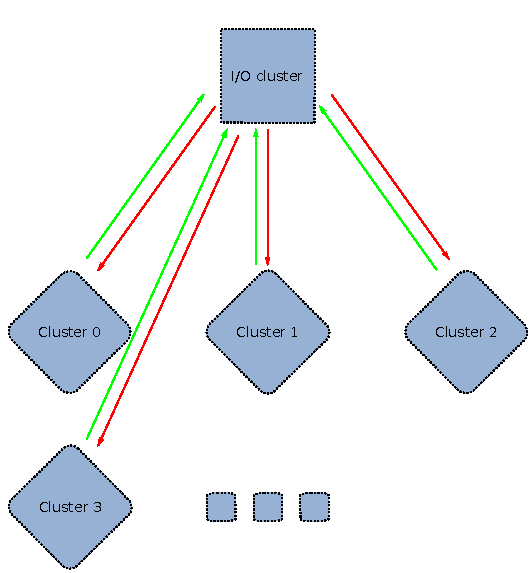
\includegraphics[width=0.5\textwidth]{figs/MPPAIPCTutorial.pdf} \\
    Fonte: Manual do \mppa.
	\label{fig:MPPAIPCTutorial}
\end{figure}

Um programa para o \mppa é composto por, pelo menos, dois arquivos principais:
um deles conterá o código a ser executado pelo processo mestre e outro conterá o código
a ser executado por cada processo trabalhador. Esses arquivos são compilados separadamente,
gerando dois arquivos binários (um para o processo mestre e outro para os
processos trabalhadores).
O binário dos trabalhadores é utilizado como argumento de entrada da função \texttt{MPPA\_Spawn()}
descrita anteriormente durante a criação dos processos trabalhadores.

Trabalhos anteriores mostraram que desenvolver aplicações paralelas otimizadas
para o \mppa é um grande desafio~\cite{Castro-IA3-JPDC:2014} devido a alguns
fatores importantes. O primeiro deles está relacionado ao \textbf{modelo de
    programação híbrido} exigido pelo processador: \textit{threads} em um mesmo
\textit{cluster} se comunicam através de uma memória compartilhada local, porém
a comunicação entre \textit{clusters} é feita explicitamente via \noc, em um
modelo de memória distribuída. Mais especificamente, aplicações desenvolvidas
para o \mppa precisam utilizar duas bibliotecas de programação paralela para
utilizar os recursos do processador: OpenMP, baseado em um modelo de memória
compartilhada, utilizada para paralelizar a computação dentro de cada
\textit{cluster} e a \api proprietária do \mppa, que segue um modelo de memória
distribuída, sendo utilizado na comunicação entre os \textit{clusters} e o
subsistema de \es por meio da \noc. O segundo fator importante está relacionado
à \textbf{capacidade limitada de memória} no \textit{chip}: cada \textit{cluster}
possui apenas 2~\mb de memória local de baixa latência. Portanto, aplicações
reais precisam constantemente realizar comunicações com o subsistema de \es
conectado à memória \lpddr. Por fim, o último fator está diretamente relacionado
à \textbf{ausência de coerência de \textit{cache}}: cada \pe possui uma memória
\textit{cache} privada sem coerência de \textit{cache}, sendo necessário o uso
explícito de instruções do tipo \textit{flush} para atualizar a \textit{cache}
de um \pe quando necessário.


\begin{figure}[t]
	\centering
	\caption{Ilustração do padrão \stencil.}
	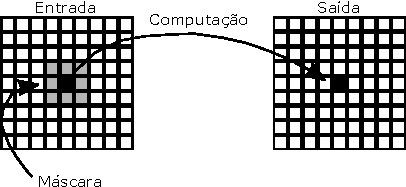
\includegraphics[width=0.6\textwidth]{figs/stencilComp.pdf} \\
    Fonte: desenvolvido pelo autor.
	\label{fig:stencil}
\end{figure}

\section{O Padrão \textit{Stencil}}
\label{sec:stencil}

As dificuldades na computação paralela proporcionam um grande impacto no desenvolvimento de aplicações. Com o
desenvolvimento de aplicações paralelas, começou-se a notar um padrão entre
elas. Com isso, foram criados os padrões paralelos para simplificar o
desenvolvimento de código.
% ~\cite{Cole M. Algorithmic skeletons: structured management of parallel computations, Research monographs in parallel and distributed computing.
% London: Pitman; 1989.}
% McCool MD. Structured parallel programming with deterministic patterns. Proceedings of the 2Nd USENIX Conference on Hot Topics in Parallelism, HotPar'10, USENIX Association, Berkeley, CA, 2010; 5–5.
Para uma maior abstração e redução da complexidade dos padrões, foram propostos
esqueletos paralelos. Na programação paralela com esqueletos, o esqueleto é responsável por
gerenciar o controle de tarefas e dados, retirando essa responsabilidade do
desenvolvedor. Desta forma, é possível simplificar grande parte do
desenvolvimento de aplicações paralelas e auxiliar em outras funções que podem
trazer uma maior dificuldade ao desenvolvedor. Mais especificamente, o
desenvolvedor irá focar apenas em especificar o algoritmo, deixando o esqueleto
gerenciar os detalhes de execução, diminuindo o tempo de desenvolvimento e
\textit{debug} da aplicação.

Existem diversos padrões paralelos, como o \textit{map}, \textit{reduce},
\textit{scan}, \stencil, entre outros. Dentre os padrões existentes, o
padrão \stencil é de grande importância tanto no ambiente acadêmico quanto no
industrial, utilizado em diversos campos importantes, como física quântica,
previsão do tempo e processamento de imagens~\cite{pereira15}.

\begin{figure}[t]
	\begin{lstlisting}[
		caption=Exemplo de código \stencil (aplicação Jacobi).,
		label=cod:exemplo-stencil,
	]
	void jacobi(int tsteps, int N, float *A, float *B){
		int t, i, j;
		float c1 = 0.2;

		for (t = 0; t < tsteps; t++){
			for (i = 1; i < N-1; i++)
				for (j = 1; j < N-1; j++)
					B[i,j] = c1 * (A[i,j] + A[i,j-1] + A[i,j+1] + A[i+1,j]
                         + A[i-1,j]);

			for (i = 1; i < N-1; i++)
				for (j = 1; j < N-1; j++)
					A[i,j] = B[i,j]
		}
	}
\end{lstlisting}
\end{figure}

O padrão \stencil atualiza elementos de uma matriz de entrada ($A$),
de acordo com um padrão especificado. Mais especificamente, em uma aplicação
\stencil, cada iteração utiliza a máscara de vizinhança responsável por determinar os vizinhos
utilizados na computação. A máscara é aplicada sobre $A$ para determinar o valor de cada
célula da matriz de saída ($B$). No exemplo da Figura~\ref{fig:stencil}, o
valor de cada célula da matriz de saída é determinado em função dos
valores de cada uma das células vizinhas adjacentes da matriz de entrada. Esse processo é realizado
para todas as células da matriz de entrada, produzindo uma matriz de saída
contendo o resultado da computação \stencil. Além disso, o padrão possibilita a computação
iterativa, isto é, ao final de uma iteração, a matriz de saída será
considerada como a matriz de entrada para a próxima iteração,
caracterizando uma nova iteração da computação.

O Código~\ref{cod:exemplo-stencil} apresenta um exemplo do código de uma aplicação baseada no padrão
\stencil, cujo o objetivo é a realização da resolução de equações matriciais pelo método iterativo de Jacobi.
O número de iterações é determinado pelo parâmetro \texttt{tsteps} (linha 5). A computação
\stencil é realizada lendo-se as informações da matriz de entrada \texttt{A} e escrevendo-se os resultados em uma matriz de saída \texttt{B}, ambas de tamanho \texttt{N*N}.
Nesse exemplo, foi utilizado um coeficiente \texttt{c1} e uma vizinhança de 5 elementos (linha 8). A vizinhança de 5 elementos
representa a célula central e as 4 células adjacentes à célula central (cima, baixo, esquerda e direita).
Devido à característica iterativa desta aplicação, existe uma troca de dados entre as matrizes \texttt{A} e \texttt{B}
(linhas 10-12) para que o resultado da iteração \texttt{i} possa ser utilizado como entrada na iteração
\texttt{i+1}.

% \todo[inline]{- Adicionar 1 ou 2 parágrafos falando de exemplos de aplicações que usam esse padrão.
% Podes usar o Fur e o Jacobi.}

\section{PSkel}
\label{sec:pskel}

O \pskel é um \fw de programação em alto nível para o padrão \stencil, que
oferece suporte a execuções paralelas em arquiteturas heterogêneas incluindo \cpu
e \gpu. Utilizando uma única interface de programação escrita em C++, o usuário é
responsável por definir o \textit{kernel} principal da computação \stencil,
enquanto o \fw se encarrega de gerar código executável para as diferentes
plataformas paralelas e realizar todo o gerenciamento de memória e transferência
de dados entre dispositivos de forma transparente~\cite{pereira15}. Mais
especificamente, o \pskel traduz as abstrações em código C++ de baixo nível,
compatível com Intel TBB e NVIDIA CUDA.

A \api do PSkel possibilita a definição de \textit{templates} para a manipulação
de estruturas $n$-dimensionais, denominadas \texttt{Array} (1 dimensão),
\texttt{Array2D} (2 dimensões) e \texttt{Array3D} (3 dimensões). Além disso, o
\fw provê abstrações para a definição da vizinhança do \stencil (máscara)
e o \textit{kernel} da computação \stencil (\texttt{stencilKernel()}). O
\texttt{stencilKernel()} é um método a ser implementado pelo usuário que
descreve, especificamente, a computação que será executada para cada célula do
\texttt{Array} de entrada com base nos valores de sua vizinhança (máscara).

Desta forma, o desenvolvedor deverá seguir os seguintes passos para desenvolver
uma aplicação \stencil com \pskel:

\begin{enumerate}
	\item Identificar a dimensão do problema, construindo estruturas de acordo com
	os recipientes especificados pelo \fw;

	\item Definir o método \texttt{stencilKernel()} que descreve a computação executada
	sobre os elementos da máscara e do \texttt{Array} de entrada;

	\item Instanciar um ou mais objetos \texttt{Stencil} para gerenciar os encapsulamentos,
	alocação de memória e chamadas para efetuar a computação determinada pelo método
	\texttt{stencilKernel()}. Mais especificamente, os recipientes são estruturas que
	armazenam \texttt{Arrays} para leitura/escrita de dados. Eles são responsáveis por
	gerenciar a alocação de memória na \cpu e \gpu de maneira transparente.

	\item Instanciar a classe de \textit{Runtime} que adota um padrão \textit{Facade} que
	efetua a abstração dos detalhes da implementação e configurações do padrão \stencil.
	Essa classe provê os métodos de execução para os padrões \stencil, além do
	particionamento transparente de tarefas e dados entre \cpu e \gpu.
\end{enumerate}

% \begin{figure}[t]
% \centering
% 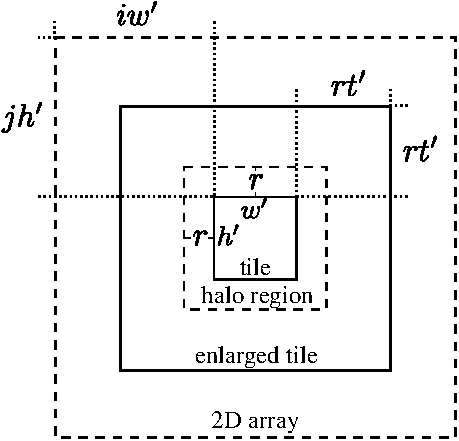
\includegraphics[width=0.3\columnwidth]{figs/tile.pdf}
% \caption{ Diagrama do \textit{tiling} 2D. Um \textit{tile} lógico (linha interna sólida) é contido dentro do Array
%     2D (linha externa pontilhada) com \textit{offsets} verticais e horizontais dado por $j  h^\prime$
%     e $i  w^\prime$. Computar $t^\prime$ consecutivas iterações stencil no \textit{tile} requer um aumento no
%     \textit{tile} lógico com uma \textit{ghost zone} (área entre a linha interna sólida e a linha externa sólida), que é constituída
%     de regiões \textit{halo} (área entre a linha interna sólida e a linha interna pontilhada).}
% \label{fig:gputile}
% %\vspace{-4em}
% \end{figure}
%

\begin{figure}[t]
	\begin{lstlisting}[
		caption=Exemplo do código da aplicação Jacobi no PSkel.,
		label=cod:exemplo-pskel,
	]
	__parallel__ void
	stencilKernel(Array2D<float> A, Array2D<float> B, Mask2D<int> mask,
								struct Arguments args, int x, int y){
		B(x,y) = args.alpha * (A(x,y) + A(x,y+1) + A(x,y-1) + A(x+1,y)
                           + A(x-1,y));
	}

	int main(int argc, char **argv) {
		/* declaracoes de variaveis omitidas */

		Array2D<float> input(A, M, N);
		Array2D<float> output(B, M, N);
		int neighbors = {{0,1}, {-1,0}, {1,0}, {-1,0}};
		Mask2D<int> mask(4, neighbors);
		struct Arguments args(alpha);

		Stencil2D<Array2D<float>, Mask2D<int>, Arguments>
			jacobi(A, B, args);
		jacobi.runIterative(device::GPU, tsteps, 1.0);

		return(0);
	}
\end{lstlisting}
\end{figure}

Em uma aplicação \stencil iterativa, cada iteração utiliza a máscara de
vizinhança sobre o \texttt{Array} de entrada para determinar o
valor de cada célula do \texttt{Array} de saída. No exemplo da
Figura~\ref{fig:stencil}, o valor de cada célula do \texttt{Array} de saída é
determinado em função dos valores de cada uma das células vizinhas adjacentes.
Esse processo é realizado para todas as células do \texttt{Array} de entrada,
produzindo um \texttt{Array} de saída da computação \textit{stencil}. Ao final de uma
iteração, o \texttt{Array} de saída será considerado como \texttt{Array} de
entrada para a próxima iteração no caso de uma aplicação \textit{stencil} iterativa.

O Código~\ref{cod:exemplo-pskel} apresenta um exemplo da aplicação Jacobi discutida na
Seção~\ref{sec:stencil} (Código~\ref{cod:exemplo-stencil}), porém agora implementada no \fw \pskel.
Nesse exemplo, a função \stencil principal da aplicação está implementada no método \texttt{stencilKernel()} nas linhas 1-5.
As estruturas para efetuar a computação, como o \texttt{Array} de entrada (\texttt{input}) e de saída (\texttt{output}), são mostrados nas linhas 10-11.
O formato da vizinhança é especificado na linha 12, sendo guardado na variável \texttt{neighbors}.
Então, a máscara é construída na linha 13 com base na vizinhança definida anteriormente.
Estruturas como \texttt{Array2D}, \texttt{Mask2D}, são exemplos dos
recipientes disponibilizados pelo \fw. A classe de \textit{runtime} é
determinada pela estrutura \texttt{Stencil2D} (linha 16), onde ao efetuar a chamada para
função \texttt{runIterative()} (linha 18), a execução da computação irá iniciar.

% \todo[inline]{Falar mais precisamente o que é feito em cada linha.}

É possível notar que o \textit{kernel} da computação \stencil (linha 4) fica mais simplificado em relação ao
código original do Jacobi mostrado anteriormente (Código~\ref{cod:exemplo-stencil}), pois as iterações da aplicação
(\texttt{tsteps}) e os laços de computação sobre as matrizes ficam implícitos, sendo
gerenciados pelo \fw. Os elementos das matrizes são determinados pelos
parâmetros \texttt{x} e \texttt{y} da função \texttt{stencilKernel()}. Além disso, o coeficiente
da aplicação Jacobi é passado como parâmetro por uma \texttt{struct} denominada
\texttt{Arguments} (linha 14).


